\documentclass[12pt]{article}
\usepackage[
  top=2.50cm,
  bottom=1.50cm,
  left=1.50cm,
  right=1.50cm
]{geometry} 
\usepackage{amsmath,amsthm,amssymb}
\usepackage{algorithm,algorithmic}
\usepackage{graphicx}
\usepackage{tikz}

\newenvironment{theorem}[2][Theorem]{\begin{trivlist}
\item[\hskip \labelsep {\bfseries #1}\hskip \labelsep {\bfseries #2.}]}{\end{trivlist}}
\newenvironment{lemma}[2][Lemma]{\begin{trivlist}
\item[\hskip \labelsep {\bfseries #1}\hskip \labelsep {\bfseries #2.}]}{\end{trivlist}}
\newenvironment{exercise}[2][Exercise]{\begin{trivlist}
\item[\hskip \labelsep {\bfseries #1}\hskip \labelsep {\bfseries #2.}]}{\end{trivlist}}
\newenvironment{problem}[2][Problem]{\begin{trivlist}
\item[\hskip \labelsep {\bfseries #1}\hskip \labelsep {\bfseries #2.}]}{\end{trivlist}}
\newenvironment{question}[2][Question]{\begin{trivlist}
\item[\hskip \labelsep {\bfseries #1}\hskip \labelsep {\bfseries #2.}]}{\end{trivlist}}
\newenvironment{corollary}[2][Corollary]{\begin{trivlist}
\item[\hskip \labelsep {\bfseries #1}\hskip \labelsep {\bfseries #2.}]}{\end{trivlist}}

\begin{document}

\title{Homework 10}
\author{Thomas Kim~tsk389~51835\\David Munoz~dam2989~51840\\
CS331 Algorithms and Complexity}

\renewcommand{\arraystretch}{2.0}

\date{} % Suppress the datn{minipage}{0.5\textwidth}

% ------------------
% Begin Cover Page
% ------------------

\maketitle
% ------------------
% Begin Homework
% ------------------

\onecolumn

\begin{problem}
  {Q1(a)}
    Sort the following list of functions in ascending order of growth rates.\\
    % TODO: order these
      \begin{enumerate}
        \item $f_7(n) = \sqrt{n}$
        \item $f_4(n) = n(logn)^3$
        \item $f_5(n) = n^4$
        \item $f_6(n) = 2^{2^{log(logn)}}$
        \item $f_3(n) = n^{logn}$
        \item $f_2(n) = 2^{n^3}$
        \item $f_1(n) = 2^{2^n}$
      \end{enumerate}
\end{problem}

\begin{problem}
  {Q1(b)}
  Consider a network $G = (V,E)$ with a source $s$, a sink $t$, and a capacity $c_e$ on every edge $e \in E$. \\
  Claim: if $f$ is a maximum $s-t$ flow in $G$, then $f$ either saturates every edge out of $s$ or saturates every edge into $t$. \\
  \textbf{False} \\
  \begin{proof}
  \begin{center}
  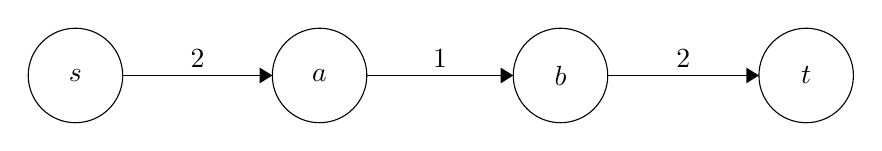
\begin{tikzpicture}[scale=0.2]
  \tikzstyle{every node}+=[inner sep=0pt]
  \draw [black] (8.5,-30.9) circle (3);
  \draw (8.5,-30.9) node {$s$};
  \draw [black] (24,-30.9) circle (3);
  \draw (24,-30.9) node {$a$};
  \draw [black] (39.3,-30.9) circle (3);
  \draw (39.3,-30.9) node {$b$};
  \draw [black] (54.9,-30.9) circle (3);
  \draw (54.9,-30.9) node {$t$};
  \draw [black] (11.5,-30.9) -- (21,-30.9);
  \fill [black] (21,-30.9) -- (20.2,-30.4) -- (20.2,-31.4);
  \draw (16.25,-30.4) node [above] {$2$};
  \draw [black] (27,-30.9) -- (36.3,-30.9);
  \fill [black] (36.3,-30.9) -- (35.5,-30.4) -- (35.5,-31.4);
  \draw (31.65,-30.4) node [above] {$1$};
  \draw [black] (42.3,-30.9) -- (51.9,-30.9);
  \fill [black] (51.9,-30.9) -- (51.1,-30.4) -- (51.1,-31.4);
  \draw (47.1,-30.4) node [above] {$2$};
  \end{tikzpicture}
  \end{center}
  The min cut is $A = \{s,a\}, B = \{b,t\}$. The value of this cut is $1$, which implies the max flow $f = 1$. This does not saturate the edge leaving $s$ or the edge entering $t$. \\
  \end{proof}
\end{problem}

\begin{problem}
  {Q2}
\end{problem}

\begin{problem}
    {Q3}
    Show that the following problem is undecidable. \\
    \begin{align*}
        \textbf{A} = \{<M> | \forall w \in \textbf{S}~M \text{accepts} w\} \text{ where \textbf{S} is the set of all strings}
    \end{align*}
    \begin{proof}
        Define a mapping reduction $R(<M>)$ as follows: \\\\
        1. Erase the tape \\
        2. Write $\epsilon$ to the tape \\
        3. Run $M$ on $\epsilon$ \\
        4. Accept \\
        Return $<M\#>$ \\\\
        %% TODO: Not sure what we're allowed to reduce to
        If $<M> \in H_\epsilon: M$ halts on $\epsilon$, so $M\#$ accepts everything. Oracle $<M\#>$ accepts. \\
        If $<M> \not\in H_\epsilon: M$ does not halt on $\epsilon$, so $M\#$ accepts nothing and doesn't halt. Oracle $<M\#>$ rejects. \\
        However, no machine to decide $H$ can exist, so Oracle doesn't exist. \\
    \end{proof}
\end{problem}

\begin{problem}
    {Q4(a)}
    Given $n$ containers of weight $w_1, \dots, w_n$, trucks of capacity $K$, minimize the number of trucks to carry all the weight. This problem is NP-Complete. \\
    Greedy Algorithm: Start with an empty truck, then begin piling containers $1, 2, 3, \dots$ until you get to a container which would overflow the weight limit. \\
    Now declare this truck "loaded" and send it off; then continue the process with a fresh truck. \\
    Given an example of a set of weights, a value of $K$, where this algorithm does not use the minimum possible number of trucks. \\
\end{problem}

\begin{problem}
    {Q4(b)}
    Show, however, that the number of trucks used by this algorithm is within a factor of $2$ of the minimum possible number, for any set of weights and any value $K$ \\
\end{problem}


% -----------------
% End Homework
% -----------------

\end{document}
